\documentclass[1p]{elsarticle_modified}
%\bibliographystyle{elsarticle-num}

%\usepackage[colorlinks]{hyperref}
%\usepackage{abbrmath_seonhwa} %\Abb, \Ascr, \Acal ,\Abf, \Afrak
\usepackage{amsfonts}
\usepackage{amssymb}
\usepackage{amsmath}
\usepackage{amsthm}
\usepackage{scalefnt}
\usepackage{amsbsy}
\usepackage{kotex}
\usepackage{caption}
\usepackage{subfig}
\usepackage{color}
\usepackage{graphicx}
\usepackage{xcolor} %% white, black, red, green, blue, cyan, magenta, yellow
\usepackage{float}
\usepackage{setspace}
\usepackage{hyperref}

\usepackage{tikz}
\usetikzlibrary{arrows}

\usepackage{multirow}
\usepackage{array} % fixed length table
\usepackage{hhline}

%%%%%%%%%%%%%%%%%%%%%
\makeatletter
\renewcommand*\env@matrix[1][\arraystretch]{%
	\edef\arraystretch{#1}%
	\hskip -\arraycolsep
	\let\@ifnextchar\new@ifnextchar
	\array{*\c@MaxMatrixCols c}}
\makeatother %https://tex.stackexchange.com/questions/14071/how-can-i-increase-the-line-spacing-in-a-matrix
%%%%%%%%%%%%%%%

\usepackage[normalem]{ulem}

\newcommand{\msout}[1]{\ifmmode\text{\sout{\ensuremath{#1}}}\else\sout{#1}\fi}
%SOURCE: \msout is \stkout macro in https://tex.stackexchange.com/questions/20609/strikeout-in-math-mode

\newcommand{\cancel}[1]{
	\ifmmode
	{\color{red}\msout{#1}}
	\else
	{\color{red}\sout{#1}}
	\fi
}

\newcommand{\add}[1]{
	{\color{blue}\uwave{#1}}
}

\newcommand{\replace}[2]{
	\ifmmode
	{\color{red}\msout{#1}}{\color{blue}\uwave{#2}}
	\else
	{\color{red}\sout{#1}}{\color{blue}\uwave{#2}}
	\fi
}

\newcommand{\Sol}{\mathcal{S}} %segment
\newcommand{\D}{D} %diagram
\newcommand{\A}{\mathcal{A}} %arc


%%%%%%%%%%%%%%%%%%%%%%%%%%%%%5 test

\def\sl{\operatorname{\textup{SL}}(2,\Cbb)}
\def\psl{\operatorname{\textup{PSL}}(2,\Cbb)}
\def\quan{\mkern 1mu \triangleright \mkern 1mu}

\theoremstyle{definition}
\newtheorem{thm}{Theorem}[section]
\newtheorem{prop}[thm]{Proposition}
\newtheorem{lem}[thm]{Lemma}
\newtheorem{ques}[thm]{Question}
\newtheorem{cor}[thm]{Corollary}
\newtheorem{defn}[thm]{Definition}
\newtheorem{exam}[thm]{Example}
\newtheorem{rmk}[thm]{Remark}
\newtheorem{alg}[thm]{Algorithm}

\newcommand{\I}{\sqrt{-1}}
\begin{document}

%\begin{frontmatter}
%
%\title{Boundary parabolic representations of knots up to 8 crossings}
%
%%% Group authors per affiliation:
%\author{Yunhi Cho} 
%\address{Department of Mathematics, University of Seoul, Seoul, Korea}
%\ead{yhcho@uos.ac.kr}
%
%
%\author{Seonhwa Kim} %\fnref{s_kim}}
%\address{Center for Geometry and Physics, Institute for Basic Science, Pohang, 37673, Korea}
%\ead{ryeona17@ibs.re.kr}
%
%\author{Hyuk Kim}
%\address{Department of Mathematical Sciences, Seoul National University, Seoul 08826, Korea}
%\ead{hyukkim@snu.ac.kr}
%
%\author{Seokbeom Yoon}
%\address{Department of Mathematical Sciences, Seoul National University, Seoul, 08826,  Korea}
%\ead{sbyoon15@snu.ac.kr}
%
%\begin{abstract}
%We find all boundary parabolic representation of knots up to 8 crossings.
%
%\end{abstract}
%\begin{keyword}
%    \MSC[2010] 57M25 
%\end{keyword}
%
%\end{frontmatter}

%\linenumbers
%\tableofcontents
%
\newcommand\colored[1]{\textcolor{white}{\rule[-0.35ex]{0.8em}{1.4ex}}\kern-0.8em\color{red} #1}%
%\newcommand\colored[1]{\textcolor{white}{ #1}\kern-2.17ex	\textcolor{white}{ #1}\kern-1.81ex	\textcolor{white}{ #1}\kern-2.15ex\color{red}#1	}

{\Large $\underline{11a_{181}~(K11a_{181})}$}

\setlength{\tabcolsep}{10pt}
\renewcommand{\arraystretch}{1.6}
\vspace{1cm}\begin{tabular}{m{100pt}>{\centering\arraybackslash}m{274pt}}
\multirow{5}{120pt}{
	\centering
	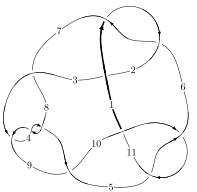
\includegraphics[width=112pt]{../../../GIT/diagram.site/Diagrams/png/430_11a_181.png}\\
\ \ \ A knot diagram\footnotemark}&
\allowdisplaybreaks
\textbf{Linearized knot diagam} \\
\cline{2-2}
 &
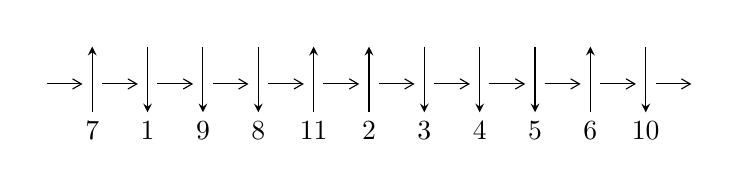
\begin{tikzpicture}[x=20pt, y=17pt]
	% nodes
	\node (C0) at (0, 0) {};
	\node (C1) at (1, 0) {};
	\node (C1U) at (1, +1) {};
	\node (C1D) at (1, -1) {7};

	\node (C2) at (2, 0) {};
	\node (C2U) at (2, +1) {};
	\node (C2D) at (2, -1) {1};

	\node (C3) at (3, 0) {};
	\node (C3U) at (3, +1) {};
	\node (C3D) at (3, -1) {9};

	\node (C4) at (4, 0) {};
	\node (C4U) at (4, +1) {};
	\node (C4D) at (4, -1) {8};

	\node (C5) at (5, 0) {};
	\node (C5U) at (5, +1) {};
	\node (C5D) at (5, -1) {11};

	\node (C6) at (6, 0) {};
	\node (C6U) at (6, +1) {};
	\node (C6D) at (6, -1) {2};

	\node (C7) at (7, 0) {};
	\node (C7U) at (7, +1) {};
	\node (C7D) at (7, -1) {3};

	\node (C8) at (8, 0) {};
	\node (C8U) at (8, +1) {};
	\node (C8D) at (8, -1) {4};

	\node (C9) at (9, 0) {};
	\node (C9U) at (9, +1) {};
	\node (C9D) at (9, -1) {5};

	\node (C10) at (10, 0) {};
	\node (C10U) at (10, +1) {};
	\node (C10D) at (10, -1) {6};

	\node (C11) at (11, 0) {};
	\node (C11U) at (11, +1) {};
	\node (C11D) at (11, -1) {10};
	\node (C12) at (12, 0) {};

	% arrows
	\draw[->,>={angle 60}]
	(C0) edge (C1) (C1) edge (C2) (C2) edge (C3) (C3) edge (C4) (C4) edge (C5) (C5) edge (C6) (C6) edge (C7) (C7) edge (C8) (C8) edge (C9) (C9) edge (C10) (C10) edge (C11) (C11) edge (C12) ;	\draw[->,>=stealth]
	(C1D) edge (C1U) (C2U) edge (C2D) (C3U) edge (C3D) (C4U) edge (C4D) (C5D) edge (C5U) (C6D) edge (C6U) (C7U) edge (C7D) (C8U) edge (C8D) (C9U) edge (C9D) (C10D) edge (C10U) (C11U) edge (C11D) ;
	\end{tikzpicture} \\
\hhline{~~} \\& 
\textbf{Solving Sequence} \\ \cline{2-2} 
 &
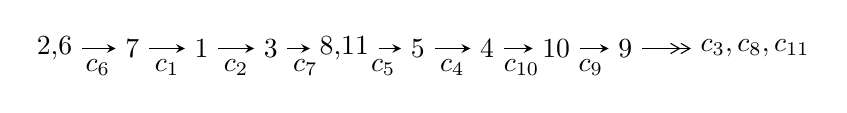
\begin{tikzpicture}[x=25pt, y=7pt]
	% node
	\node (A0) at (-1/8, 0) {2,6};
	\node (A1) at (1, 0) {7};
	\node (A2) at (2, 0) {1};
	\node (A3) at (3, 0) {3};
	\node (A4) at (65/16, 0) {8,11};
	\node (A5) at (41/8, 0) {5};
	\node (A6) at (49/8, 0) {4};
	\node (A7) at (57/8, 0) {10};
	\node (A8) at (65/8, 0) {9};
	\node (C1) at (1/2, -1) {$c_{6}$};
	\node (C2) at (3/2, -1) {$c_{1}$};
	\node (C3) at (5/2, -1) {$c_{2}$};
	\node (C4) at (7/2, -1) {$c_{7}$};
	\node (C5) at (37/8, -1) {$c_{5}$};
	\node (C6) at (45/8, -1) {$c_{4}$};
	\node (C7) at (53/8, -1) {$c_{10}$};
	\node (C8) at (61/8, -1) {$c_{9}$};
	\node (A9) at (10, 0) {$c_{3},c_{8},c_{11}$};

	% edge
	\draw[->,>=stealth]	
	(A0) edge (A1) (A1) edge (A2) (A2) edge (A3) (A3) edge (A4) (A4) edge (A5) (A5) edge (A6) (A6) edge (A7) (A7) edge (A8) ;
	\draw[->>,>={angle 60}]	
	(A8) edge (A9);
\end{tikzpicture} \\ 

\end{tabular} \\

\footnotetext{
The image of knot diagram is generated by the software ``\textbf{Draw programme}" developed by Andrew Bartholomew(\url{http://www.layer8.co.uk/maths/draw/index.htm\#Running-draw}), where we modified some parts for our purpose(\url{https://github.com/CATsTAILs/LinksPainter}).
}\phantom \\ \newline 
\centering \textbf{Ideals for irreducible components\footnotemark of $X_{\text{par}}$} 
 
\begin{align*}
I^u_{1}&=\langle 
b- u,\;u^{13}+2 u^{11}+3 u^9- u^7-4 u^3+u^2+2 a+u+1,\\
\phantom{I^u_{1}}&\phantom{= \langle  }u^{14}- u^{13}+4 u^{12}-4 u^{11}+9 u^{10}-9 u^9+11 u^8-11 u^7+10 u^6-10 u^5+6 u^4-5 u^3+4 u^2-2 u+1\rangle \\
I^u_{2}&=\langle 
- u^9-2 u^7- u^6-2 u^5- u^4- u^3- u^2+b-1,\;u^{11}+u^9+2 u^8+2 u^6- u^5+2 u^4- u^3+2 a+u-1,\\
\phantom{I^u_{2}}&\phantom{= \langle  }u^{12}+3 u^{10}+2 u^9+4 u^8+4 u^7+3 u^6+4 u^5+u^4+2 u^3+u^2+u+2\rangle \\
I^u_{3}&=\langle 
- u^9-4 u^7+u^6-6 u^5+3 u^4-3 u^3+3 u^2+b+u+1,\;- u^8-3 u^6-3 u^4+a+u+1,\\
\phantom{I^u_{3}}&\phantom{= \langle  }u^{10}- u^9+4 u^8-4 u^7+6 u^6-6 u^5+3 u^4-3 u^3+1\rangle \\
I^u_{4}&=\langle 
- u^4- u^3-2 u^2+b- a- u-1,\;2 u^4 a+2 u^3 a+u^4+4 u^2 a+a^2+3 a u+2 u^2+2 a- u,\\
\phantom{I^u_{4}}&\phantom{= \langle  }u^5+u^4+2 u^3+u^2+u+1\rangle \\
I^u_{5}&=\langle 
b- u,\;-2 u^4-2 u^3-2 u^2+a- u,\;u^5+u^4+2 u^3+u^2+u+1\rangle \\
I^u_{6}&=\langle 
b+u,\;a+2 u-1,\;u^2+1\rangle \\
\\
\end{align*}
\raggedright * 6 irreducible components of $\dim_{\mathbb{C}}=0$, with total 53 representations.\\
\footnotetext{All coefficients of polynomials are rational numbers. But the coefficients are sometimes approximated in decimal forms when there is not enough margin.}
\newpage
\renewcommand{\arraystretch}{1}
\centering \section*{I. $I^u_{1}= \langle b- u,\;u^{13}+2 u^{11}+3 u^9- u^7-4 u^3+u^2+2 a+u+1,\;u^{14}- u^{13}+\cdots-2 u+1 \rangle$}
\flushleft \textbf{(i) Arc colorings}\\
\begin{tabular}{m{7pt} m{180pt} m{7pt} m{180pt} }
\flushright $a_{2}=$&$\begin{pmatrix}0\\u\end{pmatrix}$ \\
\flushright $a_{6}=$&$\begin{pmatrix}1\\0\end{pmatrix}$ \\
\flushright $a_{7}=$&$\begin{pmatrix}1\\- u^2\end{pmatrix}$ \\
\flushright $a_{1}=$&$\begin{pmatrix}- u\\u^3+u\end{pmatrix}$ \\
\flushright $a_{3}=$&$\begin{pmatrix}- u^3\\u^5+u^3+u\end{pmatrix}$ \\
\flushright $a_{8}=$&$\begin{pmatrix}- u^6- u^4+1\\u^8+2 u^6+2 u^4\end{pmatrix}$ \\
\flushright $a_{11}=$&$\begin{pmatrix}-\frac{1}{2} u^{13}- u^{11}+\cdots-\frac{1}{2} u-\frac{1}{2}\\u\end{pmatrix}$ \\
\flushright $a_{5}=$&$\begin{pmatrix}-\frac{1}{2} u^{13}+u^{12}+\cdots-\frac{3}{2} u+\frac{3}{2}\\u^2\end{pmatrix}$ \\
\flushright $a_{4}=$&$\begin{pmatrix}- u^5+u^4-2 u^3+u^2- u+1\\-\frac{1}{2} u^{13}-2 u^{11}+\cdots+\frac{1}{2} u+\frac{1}{2}\end{pmatrix}$ \\
\flushright $a_{10}=$&$\begin{pmatrix}-\frac{1}{2} u^{13}- u^{11}+\cdots-\frac{3}{2} u-\frac{1}{2}\\u\end{pmatrix}$ \\
\flushright $a_{9}=$&$\begin{pmatrix}-\frac{1}{2} u^{13}- u^{11}+\cdots-\frac{1}{2} u-\frac{1}{2}\\u^5+u^3+u\end{pmatrix}$\\ \flushright $a_{9}=$&$\begin{pmatrix}-\frac{1}{2} u^{13}- u^{11}+\cdots-\frac{1}{2} u-\frac{1}{2}\\u^5+u^3+u\end{pmatrix}$\\&\end{tabular}
\flushleft \textbf{(ii) Obstruction class $= -1$}\\~\\
\flushleft \textbf{(iii) Cusp Shapes $= -4 u^{13}+4 u^{12}-14 u^{11}+12 u^{10}-26 u^9+24 u^8-20 u^7+20 u^6-10 u^5+20 u^4-2 u^3-6 u$}\\~\\
\newpage\renewcommand{\arraystretch}{1}
\flushleft \textbf{(iv) u-Polynomials at the component}\newline \\
\begin{tabular}{m{50pt}|m{274pt}}
Crossings & \hspace{64pt}u-Polynomials at each crossing \\
\hline $$\begin{aligned}c_{1},c_{5},c_{6}\\c_{10}\end{aligned}$$&$\begin{aligned}
&u^{14}- u^{13}+\cdots-2 u+1
\end{aligned}$\\
\hline $$\begin{aligned}c_{2},c_{11}\end{aligned}$$&$\begin{aligned}
&u^{14}+7 u^{13}+\cdots+4 u+1
\end{aligned}$\\
\hline $$\begin{aligned}c_{3},c_{4},c_{8}\end{aligned}$$&$\begin{aligned}
&u^{14}+2 u^{13}+\cdots+3 u+2
\end{aligned}$\\
\hline $$\begin{aligned}c_{7},c_{9}\end{aligned}$$&$\begin{aligned}
&u^{14}-2 u^{13}+\cdots-12 u+8
\end{aligned}$\\
\hline
\end{tabular}\\~\\
\newpage\renewcommand{\arraystretch}{1}
\flushleft \textbf{(v) Riley Polynomials at the component}\newline \\
\begin{tabular}{m{50pt}|m{274pt}}
Crossings & \hspace{64pt}Riley Polynomials at each crossing \\
\hline $$\begin{aligned}c_{1},c_{5},c_{6}\\c_{10}\end{aligned}$$&$\begin{aligned}
&y^{14}+7 y^{13}+\cdots+4 y+1
\end{aligned}$\\
\hline $$\begin{aligned}c_{2},c_{11}\end{aligned}$$&$\begin{aligned}
&y^{14}+3 y^{13}+\cdots+28 y^2+1
\end{aligned}$\\
\hline $$\begin{aligned}c_{3},c_{4},c_{8}\end{aligned}$$&$\begin{aligned}
&y^{14}+12 y^{13}+\cdots+11 y+4
\end{aligned}$\\
\hline $$\begin{aligned}c_{7},c_{9}\end{aligned}$$&$\begin{aligned}
&y^{14}-10 y^{13}+\cdots+496 y+64
\end{aligned}$\\
\hline
\end{tabular}\\~\\
\newpage\flushleft \textbf{(vi) Complex Volumes and Cusp Shapes}
$$\begin{array}{c|c|c}  
\text{Solutions to }I^u_{1}& \I (\text{vol} + \sqrt{-1}CS) & \text{Cusp shape}\\
 \hline 
\begin{aligned}
u &= -0.460484 + 0.954971 I \\
a &= \phantom{-}1.80473 + 1.22926 I \\
b &= -0.460484 + 0.954971 I\end{aligned}
 & -1.77357 - 5.35695 I & -6.00056 + 9.03526 I \\ \hline\begin{aligned}
u &= -0.460484 - 0.954971 I \\
a &= \phantom{-}1.80473 - 1.22926 I \\
b &= -0.460484 - 0.954971 I\end{aligned}
 & -1.77357 + 5.35695 I & -6.00056 - 9.03526 I \\ \hline\begin{aligned}
u &= -0.628671 + 0.622459 I \\
a &= \phantom{-}0.748022 + 0.456292 I \\
b &= -0.628671 + 0.622459 I\end{aligned}
 & \phantom{-}5.80501 - 1.28126 I & \phantom{-}3.72038 + 3.33843 I \\ \hline\begin{aligned}
u &= -0.628671 - 0.622459 I \\
a &= \phantom{-}0.748022 - 0.456292 I \\
b &= -0.628671 - 0.622459 I\end{aligned}
 & \phantom{-}5.80501 + 1.28126 I & \phantom{-}3.72038 - 3.33843 I \\ \hline\begin{aligned}
u &= \phantom{-}0.582308 + 0.988094 I \\
a &= -1.26996 + 1.41625 I \\
b &= \phantom{-}0.582308 + 0.988094 I\end{aligned}
 & \phantom{-}3.60332 + 8.26243 I & -0.67488 - 8.53661 I \\ \hline\begin{aligned}
u &= \phantom{-}0.582308 - 0.988094 I \\
a &= -1.26996 - 1.41625 I \\
b &= \phantom{-}0.582308 - 0.988094 I\end{aligned}
 & \phantom{-}3.60332 - 8.26243 I & -0.67488 + 8.53661 I \\ \hline\begin{aligned}
u &= \phantom{-}0.799677 + 0.138430 I \\
a &= -0.192212 + 0.103093 I \\
b &= \phantom{-}0.799677 + 0.138430 I\end{aligned}
 & \phantom{-}1.59498 - 3.95770 I & \phantom{-}0.96673 + 2.71748 I \\ \hline\begin{aligned}
u &= \phantom{-}0.799677 - 0.138430 I \\
a &= -0.192212 - 0.103093 I \\
b &= \phantom{-}0.799677 - 0.138430 I\end{aligned}
 & \phantom{-}1.59498 + 3.95770 I & \phantom{-}0.96673 - 2.71748 I \\ \hline\begin{aligned}
u &= \phantom{-}0.492502 + 1.221530 I \\
a &= -1.29138 + 2.41020 I \\
b &= \phantom{-}0.492502 + 1.221530 I\end{aligned}
 & -9.30050 + 9.21742 I & -9.53627 - 6.56177 I \\ \hline\begin{aligned}
u &= \phantom{-}0.492502 - 1.221530 I \\
a &= -1.29138 - 2.41020 I \\
b &= \phantom{-}0.492502 - 1.221530 I\end{aligned}
 & -9.30050 - 9.21742 I & -9.53627 + 6.56177 I\\
 \hline 
 \end{array}$$\newpage$$\begin{array}{c|c|c}  
\text{Solutions to }I^u_{1}& \I (\text{vol} + \sqrt{-1}CS) & \text{Cusp shape}\\
 \hline 
\begin{aligned}
u &= -0.525386 + 1.228370 I \\
a &= \phantom{-}1.17574 + 2.34936 I \\
b &= -0.525386 + 1.228370 I\end{aligned}
 & -4.8439 - 13.8790 I & -5.49540 + 8.77072 I \\ \hline\begin{aligned}
u &= -0.525386 - 1.228370 I \\
a &= \phantom{-}1.17574 - 2.34936 I \\
b &= -0.525386 - 1.228370 I\end{aligned}
 & -4.8439 + 13.8790 I & -5.49540 - 8.77072 I \\ \hline\begin{aligned}
u &= \phantom{-}0.240054 + 0.605061 I \\
a &= -0.974923 - 0.634482 I \\
b &= \phantom{-}0.240054 + 0.605061 I\end{aligned}
 & -0.020113 + 1.303980 I & -0.98002 - 6.02630 I \\ \hline\begin{aligned}
u &= \phantom{-}0.240054 - 0.605061 I \\
a &= -0.974923 + 0.634482 I \\
b &= \phantom{-}0.240054 - 0.605061 I\end{aligned}
 & -0.020113 - 1.303980 I & -0.98002 + 6.02630 I\\
 \hline 
 \end{array}$$\newpage\newpage\renewcommand{\arraystretch}{1}
\centering \section*{II. $I^u_{2}= \langle - u^9-2 u^7- u^6-2 u^5- u^4- u^3- u^2+b-1,\;u^{11}+u^9+\cdots+2 a-1,\;u^{12}+3 u^{10}+\cdots+u+2 \rangle$}
\flushleft \textbf{(i) Arc colorings}\\
\begin{tabular}{m{7pt} m{180pt} m{7pt} m{180pt} }
\flushright $a_{2}=$&$\begin{pmatrix}0\\u\end{pmatrix}$ \\
\flushright $a_{6}=$&$\begin{pmatrix}1\\0\end{pmatrix}$ \\
\flushright $a_{7}=$&$\begin{pmatrix}1\\- u^2\end{pmatrix}$ \\
\flushright $a_{1}=$&$\begin{pmatrix}- u\\u^3+u\end{pmatrix}$ \\
\flushright $a_{3}=$&$\begin{pmatrix}- u^3\\u^5+u^3+u\end{pmatrix}$ \\
\flushright $a_{8}=$&$\begin{pmatrix}- u^6- u^4+1\\u^8+2 u^6+2 u^4\end{pmatrix}$ \\
\flushright $a_{11}=$&$\begin{pmatrix}-\frac{1}{2} u^{11}-\frac{1}{2} u^9+\cdots-\frac{1}{2} u+\frac{1}{2}\\u^9+2 u^7+u^6+2 u^5+u^4+u^3+u^2+1\end{pmatrix}$ \\
\flushright $a_{5}=$&$\begin{pmatrix}-\frac{1}{2} u^{11}- u^{10}+\cdots-\frac{1}{2} u-\frac{1}{2}\\- u^{10}-2 u^8- u^7-2 u^6- u^5- u^4- u^3- u^2- u-1\end{pmatrix}$ \\
\flushright $a_{4}=$&$\begin{pmatrix}-\frac{1}{2} u^{11}-\frac{1}{2} u^9+\cdots-\frac{1}{2} u+\frac{1}{2}\\- u^{11}-3 u^9-4 u^7- u^5- u^4+u^3-2 u^2+u-1\end{pmatrix}$ \\
\flushright $a_{10}=$&$\begin{pmatrix}-\frac{1}{2} u^{11}-\frac{3}{2} u^9+\cdots-\frac{1}{2} u-\frac{1}{2}\\u^9+2 u^7+u^6+2 u^5+u^4+u^3+u^2+1\end{pmatrix}$ \\
\flushright $a_{9}=$&$\begin{pmatrix}\frac{1}{2} u^{11}+u^{10}+\cdots+\frac{3}{2} u+\frac{1}{2}\\u^{10}+u^9+2 u^8+2 u^7+3 u^6+u^5+u^4+u^2+u+1\end{pmatrix}$\\ \flushright $a_{9}=$&$\begin{pmatrix}\frac{1}{2} u^{11}+u^{10}+\cdots+\frac{3}{2} u+\frac{1}{2}\\u^{10}+u^9+2 u^8+2 u^7+3 u^6+u^5+u^4+u^2+u+1\end{pmatrix}$\\&\end{tabular}
\flushleft \textbf{(ii) Obstruction class $= -1$}\\~\\
\flushleft \textbf{(iii) Cusp Shapes $= -4 u^{10}-4 u^9-8 u^8-16 u^7-8 u^6-16 u^5-4 u^4-4 u^3-10$}\\~\\
\newpage\renewcommand{\arraystretch}{1}
\flushleft \textbf{(iv) u-Polynomials at the component}\newline \\
\begin{tabular}{m{50pt}|m{274pt}}
Crossings & \hspace{64pt}u-Polynomials at each crossing \\
\hline $$\begin{aligned}c_{1},c_{5},c_{6}\\c_{10}\end{aligned}$$&$\begin{aligned}
&u^{12}+3 u^{10}+2 u^9+4 u^8+4 u^7+3 u^6+4 u^5+u^4+2 u^3+u^2+u+2
\end{aligned}$\\
\hline $$\begin{aligned}c_{2},c_{11}\end{aligned}$$&$\begin{aligned}
&u^{12}+6 u^{11}+\cdots+3 u+4
\end{aligned}$\\
\hline $$\begin{aligned}c_{3},c_{4},c_{8}\end{aligned}$$&$\begin{aligned}
&(u^6+3 u^4+u^3+2 u^2+2 u-1)^2
\end{aligned}$\\
\hline $$\begin{aligned}c_{7},c_{9}\end{aligned}$$&$\begin{aligned}
&(u^6+3 u^5+2 u^4+u^3+5 u^2+3 u-2)^2
\end{aligned}$\\
\hline
\end{tabular}\\~\\
\newpage\renewcommand{\arraystretch}{1}
\flushleft \textbf{(v) Riley Polynomials at the component}\newline \\
\begin{tabular}{m{50pt}|m{274pt}}
Crossings & \hspace{64pt}Riley Polynomials at each crossing \\
\hline $$\begin{aligned}c_{1},c_{5},c_{6}\\c_{10}\end{aligned}$$&$\begin{aligned}
&y^{12}+6 y^{11}+\cdots+3 y+4
\end{aligned}$\\
\hline $$\begin{aligned}c_{2},c_{11}\end{aligned}$$&$\begin{aligned}
&y^{12}-2 y^{11}+\cdots- y+16
\end{aligned}$\\
\hline $$\begin{aligned}c_{3},c_{4},c_{8}\end{aligned}$$&$\begin{aligned}
&(y^6+6 y^5+13 y^4+9 y^3-6 y^2-8 y+1)^2
\end{aligned}$\\
\hline $$\begin{aligned}c_{7},c_{9}\end{aligned}$$&$\begin{aligned}
&(y^6-5 y^5+8 y^4-3 y^3+11 y^2-29 y+4)^2
\end{aligned}$\\
\hline
\end{tabular}\\~\\
\newpage\flushleft \textbf{(vi) Complex Volumes and Cusp Shapes}
$$\begin{array}{c|c|c}  
\text{Solutions to }I^u_{2}& \I (\text{vol} + \sqrt{-1}CS) & \text{Cusp shape}\\
 \hline 
\begin{aligned}
u &= -0.569850 + 0.878821 I \\
a &= \phantom{-}0.176883 - 0.327495 I \\
b &= \phantom{-}0.696319 + 0.473577 I\end{aligned}
 & \phantom{-}5.07386 - 3.39374 I & \phantom{-}2.36018 + 3.51762 I \\ \hline\begin{aligned}
u &= -0.569850 - 0.878821 I \\
a &= \phantom{-}0.176883 + 0.327495 I \\
b &= \phantom{-}0.696319 - 0.473577 I\end{aligned}
 & \phantom{-}5.07386 + 3.39374 I & \phantom{-}2.36018 - 3.51762 I \\ \hline\begin{aligned}
u &= -0.170932 + 1.042910 I \\
a &= -0.32398 - 1.97668 I \\
b &= -0.170932 - 1.042910 I\end{aligned}
 & -3.86646\phantom{ +0.000000I} & -13.16287 + 0. I\phantom{ +0.000000I} \\ \hline\begin{aligned}
u &= -0.170932 - 1.042910 I \\
a &= -0.32398 + 1.97668 I \\
b &= -0.170932 + 1.042910 I\end{aligned}
 & -3.86646\phantom{ +0.000000I} & -13.16287 + 0. I\phantom{ +0.000000I} \\ \hline\begin{aligned}
u &= -0.885163 + 0.125190 I \\
a &= -0.598885 + 1.037840 I \\
b &= \phantom{-}0.508695 + 1.194490 I\end{aligned}
 & -1.52175 + 8.77346 I & -2.43784 - 5.90094 I \\ \hline\begin{aligned}
u &= -0.885163 - 0.125190 I \\
a &= -0.598885 - 1.037840 I \\
b &= \phantom{-}0.508695 - 1.194490 I\end{aligned}
 & -1.52175 - 8.77346 I & -2.43784 + 5.90094 I \\ \hline\begin{aligned}
u &= \phantom{-}0.696319 + 0.473577 I \\
a &= \phantom{-}0.412076 + 0.210997 I \\
b &= -0.569850 + 0.878821 I\end{aligned}
 & \phantom{-}5.07386 - 3.39374 I & \phantom{-}2.36018 + 3.51762 I \\ \hline\begin{aligned}
u &= \phantom{-}0.696319 - 0.473577 I \\
a &= \phantom{-}0.412076 - 0.210997 I \\
b &= -0.569850 - 0.878821 I\end{aligned}
 & \phantom{-}5.07386 + 3.39374 I & \phantom{-}2.36018 - 3.51762 I \\ \hline\begin{aligned}
u &= \phantom{-}0.508695 + 1.194490 I \\
a &= -0.583368 - 0.583465 I \\
b &= -0.885163 + 0.125190 I\end{aligned}
 & -1.52175 + 8.77346 I & -2.43784 - 5.90094 I \\ \hline\begin{aligned}
u &= \phantom{-}0.508695 - 1.194490 I \\
a &= -0.583368 + 0.583465 I \\
b &= -0.885163 - 0.125190 I\end{aligned}
 & -1.52175 - 8.77346 I & -2.43784 + 5.90094 I\\
 \hline 
 \end{array}$$\newpage$$\begin{array}{c|c|c}  
\text{Solutions to }I^u_{2}& \I (\text{vol} + \sqrt{-1}CS) & \text{Cusp shape}\\
 \hline 
\begin{aligned}
u &= \phantom{-}0.420932 + 1.237560 I \\
a &= \phantom{-}0.66727 - 1.96181 I \\
b &= \phantom{-}0.420932 - 1.237560 I\end{aligned}
 & -9.81751\phantom{ +0.000000I} & -10.68183 + 0. I\phantom{ +0.000000I} \\ \hline\begin{aligned}
u &= \phantom{-}0.420932 - 1.237560 I \\
a &= \phantom{-}0.66727 + 1.96181 I \\
b &= \phantom{-}0.420932 + 1.237560 I\end{aligned}
 & -9.81751\phantom{ +0.000000I} & -10.68183 + 0. I\phantom{ +0.000000I}\\
 \hline 
 \end{array}$$\newpage\newpage\renewcommand{\arraystretch}{1}
\centering \section*{III. $I^u_{3}= \langle - u^9-4 u^7+\cdots+b+1,\;- u^8-3 u^6-3 u^4+a+u+1,\;u^{10}- u^9+\cdots-3 u^3+1 \rangle$}
\flushleft \textbf{(i) Arc colorings}\\
\begin{tabular}{m{7pt} m{180pt} m{7pt} m{180pt} }
\flushright $a_{2}=$&$\begin{pmatrix}0\\u\end{pmatrix}$ \\
\flushright $a_{6}=$&$\begin{pmatrix}1\\0\end{pmatrix}$ \\
\flushright $a_{7}=$&$\begin{pmatrix}1\\- u^2\end{pmatrix}$ \\
\flushright $a_{1}=$&$\begin{pmatrix}- u\\u^3+u\end{pmatrix}$ \\
\flushright $a_{3}=$&$\begin{pmatrix}- u^3\\u^5+u^3+u\end{pmatrix}$ \\
\flushright $a_{8}=$&$\begin{pmatrix}- u^6- u^4+1\\u^8+2 u^6+2 u^4\end{pmatrix}$ \\
\flushright $a_{11}=$&$\begin{pmatrix}u^8+3 u^6+3 u^4- u-1\\u^9+4 u^7- u^6+6 u^5-3 u^4+3 u^3-3 u^2- u-1\end{pmatrix}$ \\
\flushright $a_{5}=$&$\begin{pmatrix}u^7+2 u^5-2 u\\- u^9-3 u^7-3 u^5+u\end{pmatrix}$ \\
\flushright $a_{4}=$&$\begin{pmatrix}u^5- u\\- u^7- u^5+u\end{pmatrix}$ \\
\flushright $a_{10}=$&$\begin{pmatrix}- u^9+u^8-4 u^7+4 u^6-6 u^5+6 u^4-3 u^3+3 u^2\\u^9+4 u^7- u^6+6 u^5-3 u^4+3 u^3-3 u^2- u-1\end{pmatrix}$ \\
\flushright $a_{9}=$&$\begin{pmatrix}u^4+u^2-1\\- u^6-2 u^4- u^2\end{pmatrix}$\\ \flushright $a_{9}=$&$\begin{pmatrix}u^4+u^2-1\\- u^6-2 u^4- u^2\end{pmatrix}$\\&\end{tabular}
\flushleft \textbf{(ii) Obstruction class $= -1$}\\~\\
\flushleft \textbf{(iii) Cusp Shapes $= 4 u^9+12 u^7+12 u^5-4 u^3-8 u-6$}\\~\\
\newpage\renewcommand{\arraystretch}{1}
\flushleft \textbf{(iv) u-Polynomials at the component}\newline \\
\begin{tabular}{m{50pt}|m{274pt}}
Crossings & \hspace{64pt}u-Polynomials at each crossing \\
\hline $$\begin{aligned}c_{1},c_{3},c_{4}\\c_{6},c_{8}\end{aligned}$$&$\begin{aligned}
&u^{10}- u^9+4 u^8-4 u^7+6 u^6-6 u^5+3 u^4-3 u^3+1
\end{aligned}$\\
\hline $$\begin{aligned}c_{2}\end{aligned}$$&$\begin{aligned}
&u^{10}+7 u^9+20 u^8+26 u^7+6 u^6-22 u^5-19 u^4+3 u^3+6 u^2+1
\end{aligned}$\\
\hline $$\begin{aligned}c_{5},c_{10}\end{aligned}$$&$\begin{aligned}
&(u^5+u^4+2 u^3+u^2+u+1)^2
\end{aligned}$\\
\hline $$\begin{aligned}c_{7},c_{9}\end{aligned}$$&$\begin{aligned}
&(u^5- u^4-2 u^3+u^2+u+1)^2
\end{aligned}$\\
\hline $$\begin{aligned}c_{11}\end{aligned}$$&$\begin{aligned}
&(u^5+3 u^4+4 u^3+u^2- u-1)^2
\end{aligned}$\\
\hline
\end{tabular}\\~\\
\newpage\renewcommand{\arraystretch}{1}
\flushleft \textbf{(v) Riley Polynomials at the component}\newline \\
\begin{tabular}{m{50pt}|m{274pt}}
Crossings & \hspace{64pt}Riley Polynomials at each crossing \\
\hline $$\begin{aligned}c_{1},c_{3},c_{4}\\c_{6},c_{8}\end{aligned}$$&$\begin{aligned}
&y^{10}+7 y^9+20 y^8+26 y^7+6 y^6-22 y^5-19 y^4+3 y^3+6 y^2+1
\end{aligned}$\\
\hline $$\begin{aligned}c_{2}\end{aligned}$$&$\begin{aligned}
&y^{10}-9 y^9+\cdots+12 y+1
\end{aligned}$\\
\hline $$\begin{aligned}c_{5},c_{10}\end{aligned}$$&$\begin{aligned}
&(y^5+3 y^4+4 y^3+y^2- y-1)^2
\end{aligned}$\\
\hline $$\begin{aligned}c_{7},c_{9}\end{aligned}$$&$\begin{aligned}
&(y^5-5 y^4+8 y^3-3 y^2- y-1)^2
\end{aligned}$\\
\hline $$\begin{aligned}c_{11}\end{aligned}$$&$\begin{aligned}
&(y^5- y^4+8 y^3-3 y^2+3 y-1)^2
\end{aligned}$\\
\hline
\end{tabular}\\~\\
\newpage\flushleft \textbf{(vi) Complex Volumes and Cusp Shapes}
$$\begin{array}{c|c|c}  
\text{Solutions to }I^u_{3}& \I (\text{vol} + \sqrt{-1}CS) & \text{Cusp shape}\\
 \hline 
\begin{aligned}
u &= \phantom{-}0.839548 + 0.070481 I \\
a &= \phantom{-}0.727084 + 1.100860 I \\
b &= -0.455697 + 1.200150 I\end{aligned}
 & -5.87256 - 4.40083 I & -6.74431 + 3.49859 I \\ \hline\begin{aligned}
u &= \phantom{-}0.839548 - 0.070481 I \\
a &= \phantom{-}0.727084 - 1.100860 I \\
b &= -0.455697 - 1.200150 I\end{aligned}
 & -5.87256 + 4.40083 I & -6.74431 - 3.49859 I \\ \hline\begin{aligned}
u &= \phantom{-}0.090539 + 1.215350 I \\
a &= \phantom{-}0.40007 - 1.64065 I \\
b &= \phantom{-}0.339110 - 0.822375 I\end{aligned}
 & -0.32910 - 1.53058 I & -2.51511 + 4.43065 I \\ \hline\begin{aligned}
u &= \phantom{-}0.090539 - 1.215350 I \\
a &= \phantom{-}0.40007 + 1.64065 I \\
b &= \phantom{-}0.339110 + 0.822375 I\end{aligned}
 & -0.32910 + 1.53058 I & -2.51511 - 4.43065 I \\ \hline\begin{aligned}
u &= \phantom{-}0.383413 + 1.200420 I \\
a &= -0.525385 - 0.755924 I \\
b &= -0.766826\phantom{ +0.000000I}\end{aligned}
 & -2.40108\phantom{ +0.000000I} & -3.48114 + 0. I\phantom{ +0.000000I} \\ \hline\begin{aligned}
u &= \phantom{-}0.383413 - 1.200420 I \\
a &= -0.525385 + 0.755924 I \\
b &= -0.766826\phantom{ +0.000000I}\end{aligned}
 & -2.40108\phantom{ +0.000000I} & -3.48114 + 0. I\phantom{ +0.000000I} \\ \hline\begin{aligned}
u &= -0.383851 + 1.270630 I \\
a &= -0.67357 - 1.92134 I \\
b &= -0.455697 - 1.200150 I\end{aligned}
 & -5.87256 + 4.40083 I & -6.74431 - 3.49859 I \\ \hline\begin{aligned}
u &= -0.383851 - 1.270630 I \\
a &= -0.67357 + 1.92134 I \\
b &= -0.455697 + 1.200150 I\end{aligned}
 & -5.87256 - 4.40083 I & -6.74431 + 3.49859 I \\ \hline\begin{aligned}
u &= -0.429649 + 0.392970 I \\
a &= -0.928202 - 0.336746 I \\
b &= \phantom{-}0.339110 + 0.822375 I\end{aligned}
 & -0.32910 + 1.53058 I & -2.51511 - 4.43065 I \\ \hline\begin{aligned}
u &= -0.429649 - 0.392970 I \\
a &= -0.928202 + 0.336746 I \\
b &= \phantom{-}0.339110 - 0.822375 I\end{aligned}
 & -0.32910 - 1.53058 I & -2.51511 + 4.43065 I\\
 \hline 
 \end{array}$$\newpage\newpage\renewcommand{\arraystretch}{1}
\centering \section*{IV. $I^u_{4}= \langle - u^4- u^3-2 u^2+b- a- u-1,\;2 u^4 a+u^4+\cdots+a^2+2 a,\;u^5+u^4+2 u^3+u^2+u+1 \rangle$}
\flushleft \textbf{(i) Arc colorings}\\
\begin{tabular}{m{7pt} m{180pt} m{7pt} m{180pt} }
\flushright $a_{2}=$&$\begin{pmatrix}0\\u\end{pmatrix}$ \\
\flushright $a_{6}=$&$\begin{pmatrix}1\\0\end{pmatrix}$ \\
\flushright $a_{7}=$&$\begin{pmatrix}1\\- u^2\end{pmatrix}$ \\
\flushright $a_{1}=$&$\begin{pmatrix}- u\\u^3+u\end{pmatrix}$ \\
\flushright $a_{3}=$&$\begin{pmatrix}- u^3\\- u^4- u^3- u^2-1\end{pmatrix}$ \\
\flushright $a_{8}=$&$\begin{pmatrix}- u^3\\- u^3- u\end{pmatrix}$ \\
\flushright $a_{11}=$&$\begin{pmatrix}a\\u^4+u^3+2 u^2+a+u+1\end{pmatrix}$ \\
\flushright $a_{5}=$&$\begin{pmatrix}- u^4 a- u^3 a- u^4-2 u^2 a-2 a u-2 u^2- a+u+1\\- a u- u^2\end{pmatrix}$ \\
\flushright $a_{4}=$&$\begin{pmatrix}- u^4 a-2 u^3 a- u^4-2 u^2 a-2 a u- u^2- a+u+1\\- u^3 a-2 a u+1\end{pmatrix}$ \\
\flushright $a_{10}=$&$\begin{pmatrix}- u^4- u^3-2 u^2- u-1\\u^4+u^3+2 u^2+a+u+1\end{pmatrix}$ \\
\flushright $a_{9}=$&$\begin{pmatrix}- u^4 a+u^4+2 u^3+u^2+a+u+1\\- u^4 a+2 u^4- u^2 a+2 u^3+3 u^2+a+2 u+2\end{pmatrix}$\\ \flushright $a_{9}=$&$\begin{pmatrix}- u^4 a+u^4+2 u^3+u^2+a+u+1\\- u^4 a+2 u^4- u^2 a+2 u^3+3 u^2+a+2 u+2\end{pmatrix}$\\&\end{tabular}
\flushleft \textbf{(ii) Obstruction class $= -1$}\\~\\
\flushleft \textbf{(iii) Cusp Shapes $= -4 u^3-4 u^2-4 u-6$}\\~\\
\newpage\renewcommand{\arraystretch}{1}
\flushleft \textbf{(iv) u-Polynomials at the component}\newline \\
\begin{tabular}{m{50pt}|m{274pt}}
Crossings & \hspace{64pt}u-Polynomials at each crossing \\
\hline $$\begin{aligned}c_{1},c_{6}\end{aligned}$$&$\begin{aligned}
&(u^5+u^4+2 u^3+u^2+u+1)^2
\end{aligned}$\\
\hline $$\begin{aligned}c_{2}\end{aligned}$$&$\begin{aligned}
&(u^5+3 u^4+4 u^3+u^2- u-1)^2
\end{aligned}$\\
\hline $$\begin{aligned}c_{3},c_{4},c_{5}\\c_{8},c_{10}\end{aligned}$$&$\begin{aligned}
&u^{10}- u^9+4 u^8-4 u^7+6 u^6-6 u^5+3 u^4-3 u^3+1
\end{aligned}$\\
\hline $$\begin{aligned}c_{7},c_{9}\end{aligned}$$&$\begin{aligned}
&(u^5- u^4-2 u^3+u^2+u+1)^2
\end{aligned}$\\
\hline $$\begin{aligned}c_{11}\end{aligned}$$&$\begin{aligned}
&u^{10}+7 u^9+20 u^8+26 u^7+6 u^6-22 u^5-19 u^4+3 u^3+6 u^2+1
\end{aligned}$\\
\hline
\end{tabular}\\~\\
\newpage\renewcommand{\arraystretch}{1}
\flushleft \textbf{(v) Riley Polynomials at the component}\newline \\
\begin{tabular}{m{50pt}|m{274pt}}
Crossings & \hspace{64pt}Riley Polynomials at each crossing \\
\hline $$\begin{aligned}c_{1},c_{6}\end{aligned}$$&$\begin{aligned}
&(y^5+3 y^4+4 y^3+y^2- y-1)^2
\end{aligned}$\\
\hline $$\begin{aligned}c_{2}\end{aligned}$$&$\begin{aligned}
&(y^5- y^4+8 y^3-3 y^2+3 y-1)^2
\end{aligned}$\\
\hline $$\begin{aligned}c_{3},c_{4},c_{5}\\c_{8},c_{10}\end{aligned}$$&$\begin{aligned}
&y^{10}+7 y^9+20 y^8+26 y^7+6 y^6-22 y^5-19 y^4+3 y^3+6 y^2+1
\end{aligned}$\\
\hline $$\begin{aligned}c_{7},c_{9}\end{aligned}$$&$\begin{aligned}
&(y^5-5 y^4+8 y^3-3 y^2- y-1)^2
\end{aligned}$\\
\hline $$\begin{aligned}c_{11}\end{aligned}$$&$\begin{aligned}
&y^{10}-9 y^9+\cdots+12 y+1
\end{aligned}$\\
\hline
\end{tabular}\\~\\
\newpage\flushleft \textbf{(vi) Complex Volumes and Cusp Shapes}
$$\begin{array}{c|c|c}  
\text{Solutions to }I^u_{4}& \I (\text{vol} + \sqrt{-1}CS) & \text{Cusp shape}\\
 \hline 
\begin{aligned}
u &= \phantom{-}0.339110 + 0.822375 I \\
a &= -0.001100 - 0.646305 I \\
b &= -0.429649 + 0.392970 I\end{aligned}
 & -0.32910 + 1.53058 I & -2.51511 - 4.43065 I \\ \hline\begin{aligned}
u &= \phantom{-}0.339110 + 0.822375 I \\
a &= \phantom{-}0.51909 - 2.25462 I \\
b &= \phantom{-}0.090539 - 1.215350 I\end{aligned}
 & -0.32910 + 1.53058 I & -2.51511 - 4.43065 I \\ \hline\begin{aligned}
u &= \phantom{-}0.339110 - 0.822375 I \\
a &= -0.001100 + 0.646305 I \\
b &= -0.429649 - 0.392970 I\end{aligned}
 & -0.32910 - 1.53058 I & -2.51511 + 4.43065 I \\ \hline\begin{aligned}
u &= \phantom{-}0.339110 - 0.822375 I \\
a &= \phantom{-}0.51909 + 2.25462 I \\
b &= \phantom{-}0.090539 + 1.215350 I\end{aligned}
 & -0.32910 - 1.53058 I & -2.51511 + 4.43065 I \\ \hline\begin{aligned}
u &= -0.766826\phantom{ +0.000000I} \\
a &= -0.92066 + 1.20042 I \\
b &= \phantom{-}0.383413 + 1.200420 I\end{aligned}
 & -2.40108\phantom{ +0.000000I} & -3.48110\phantom{ +0.000000I} \\ \hline\begin{aligned}
u &= -0.766826\phantom{ +0.000000I} \\
a &= -0.92066 - 1.20042 I \\
b &= \phantom{-}0.383413 - 1.200420 I\end{aligned}
 & -2.40108\phantom{ +0.000000I} & -3.48110\phantom{ +0.000000I} \\ \hline\begin{aligned}
u &= -0.455697 + 1.200150 I \\
a &= \phantom{-}0.563037 - 0.657755 I \\
b &= \phantom{-}0.839548 + 0.070481 I\end{aligned}
 & -5.87256 - 4.40083 I & -6.74431 + 3.49859 I \\ \hline\begin{aligned}
u &= -0.455697 + 1.200150 I \\
a &= -0.66036 - 1.99887 I \\
b &= -0.383851 - 1.270630 I\end{aligned}
 & -5.87256 - 4.40083 I & -6.74431 + 3.49859 I \\ \hline\begin{aligned}
u &= -0.455697 - 1.200150 I \\
a &= \phantom{-}0.563037 + 0.657755 I \\
b &= \phantom{-}0.839548 - 0.070481 I\end{aligned}
 & -5.87256 + 4.40083 I & -6.74431 - 3.49859 I \\ \hline\begin{aligned}
u &= -0.455697 - 1.200150 I \\
a &= -0.66036 + 1.99887 I \\
b &= -0.383851 + 1.270630 I\end{aligned}
 & -5.87256 + 4.40083 I & -6.74431 - 3.49859 I\\
 \hline 
 \end{array}$$\newpage\newpage\renewcommand{\arraystretch}{1}
\centering \section*{V. $I^u_{5}= \langle b- u,\;-2 u^4-2 u^3-2 u^2+a- u,\;u^5+u^4+2 u^3+u^2+u+1 \rangle$}
\flushleft \textbf{(i) Arc colorings}\\
\begin{tabular}{m{7pt} m{180pt} m{7pt} m{180pt} }
\flushright $a_{2}=$&$\begin{pmatrix}0\\u\end{pmatrix}$ \\
\flushright $a_{6}=$&$\begin{pmatrix}1\\0\end{pmatrix}$ \\
\flushright $a_{7}=$&$\begin{pmatrix}1\\- u^2\end{pmatrix}$ \\
\flushright $a_{1}=$&$\begin{pmatrix}- u\\u^3+u\end{pmatrix}$ \\
\flushright $a_{3}=$&$\begin{pmatrix}- u^3\\- u^4- u^3- u^2-1\end{pmatrix}$ \\
\flushright $a_{8}=$&$\begin{pmatrix}- u^3\\- u^3- u\end{pmatrix}$ \\
\flushright $a_{11}=$&$\begin{pmatrix}2 u^4+2 u^3+2 u^2+u\\u\end{pmatrix}$ \\
\flushright $a_{5}=$&$\begin{pmatrix}-2 u^3- u^2-2 u-1\\u^2\end{pmatrix}$ \\
\flushright $a_{4}=$&$\begin{pmatrix}- u^4-2 u^3- u^2-2 u-1\\- u^4\end{pmatrix}$ \\
\flushright $a_{10}=$&$\begin{pmatrix}2 u^4+2 u^3+2 u^2\\u\end{pmatrix}$ \\
\flushright $a_{9}=$&$\begin{pmatrix}u^4+u^2-1\\- u^4- u^3- u^2-1\end{pmatrix}$\\ \flushright $a_{9}=$&$\begin{pmatrix}u^4+u^2-1\\- u^4- u^3- u^2-1\end{pmatrix}$\\&\end{tabular}
\flushleft \textbf{(ii) Obstruction class $= -1$}\\~\\
\flushleft \textbf{(iii) Cusp Shapes $= -4 u^3-4 u^2-4 u-6$}\\~\\
\newpage\renewcommand{\arraystretch}{1}
\flushleft \textbf{(iv) u-Polynomials at the component}\newline \\
\begin{tabular}{m{50pt}|m{274pt}}
Crossings & \hspace{64pt}u-Polynomials at each crossing \\
\hline $$\begin{aligned}c_{1},c_{3},c_{4}\\c_{5},c_{6},c_{8}\\c_{10}\end{aligned}$$&$\begin{aligned}
&u^5+u^4+2 u^3+u^2+u+1
\end{aligned}$\\
\hline $$\begin{aligned}c_{2},c_{11}\end{aligned}$$&$\begin{aligned}
&u^5+3 u^4+4 u^3+u^2- u-1
\end{aligned}$\\
\hline $$\begin{aligned}c_{7},c_{9}\end{aligned}$$&$\begin{aligned}
&u^5- u^4-2 u^3+u^2+u+1
\end{aligned}$\\
\hline
\end{tabular}\\~\\
\newpage\renewcommand{\arraystretch}{1}
\flushleft \textbf{(v) Riley Polynomials at the component}\newline \\
\begin{tabular}{m{50pt}|m{274pt}}
Crossings & \hspace{64pt}Riley Polynomials at each crossing \\
\hline $$\begin{aligned}c_{1},c_{3},c_{4}\\c_{5},c_{6},c_{8}\\c_{10}\end{aligned}$$&$\begin{aligned}
&y^5+3 y^4+4 y^3+y^2- y-1
\end{aligned}$\\
\hline $$\begin{aligned}c_{2},c_{11}\end{aligned}$$&$\begin{aligned}
&y^5- y^4+8 y^3-3 y^2+3 y-1
\end{aligned}$\\
\hline $$\begin{aligned}c_{7},c_{9}\end{aligned}$$&$\begin{aligned}
&y^5-5 y^4+8 y^3-3 y^2- y-1
\end{aligned}$\\
\hline
\end{tabular}\\~\\
\newpage\flushleft \textbf{(vi) Complex Volumes and Cusp Shapes}
$$\begin{array}{c|c|c}  
\text{Solutions to }I^u_{5}& \I (\text{vol} + \sqrt{-1}CS) & \text{Cusp shape}\\
 \hline 
\begin{aligned}
u &= \phantom{-}0.339110 + 0.822375 I \\
a &= -2.07360 + 0.14067 I \\
b &= \phantom{-}0.339110 + 0.822375 I\end{aligned}
 & -0.32910 + 1.53058 I & -2.51511 - 4.43065 I \\ \hline\begin{aligned}
u &= \phantom{-}0.339110 - 0.822375 I \\
a &= -2.07360 - 0.14067 I \\
b &= \phantom{-}0.339110 - 0.822375 I\end{aligned}
 & -0.32910 - 1.53058 I & -2.51511 + 4.43065 I \\ \hline\begin{aligned}
u &= -0.766826\phantom{ +0.000000I} \\
a &= \phantom{-}0.198937\phantom{ +0.000000I} \\
b &= -0.766826\phantom{ +0.000000I}\end{aligned}
 & -2.40108\phantom{ +0.000000I} & -3.48110\phantom{ +0.000000I} \\ \hline\begin{aligned}
u &= -0.455697 + 1.200150 I \\
a &= \phantom{-}1.47413 + 2.44394 I \\
b &= -0.455697 + 1.200150 I\end{aligned}
 & -5.87256 - 4.40083 I & -6.74431 + 3.49859 I \\ \hline\begin{aligned}
u &= -0.455697 - 1.200150 I \\
a &= \phantom{-}1.47413 - 2.44394 I \\
b &= -0.455697 - 1.200150 I\end{aligned}
 & -5.87256 + 4.40083 I & -6.74431 - 3.49859 I\\
 \hline 
 \end{array}$$\newpage\newpage\renewcommand{\arraystretch}{1}
\centering \section*{VI. $I^u_{6}= \langle b+u,\;a+2 u-1,\;u^2+1 \rangle$}
\flushleft \textbf{(i) Arc colorings}\\
\begin{tabular}{m{7pt} m{180pt} m{7pt} m{180pt} }
\flushright $a_{2}=$&$\begin{pmatrix}0\\u\end{pmatrix}$ \\
\flushright $a_{6}=$&$\begin{pmatrix}1\\0\end{pmatrix}$ \\
\flushright $a_{7}=$&$\begin{pmatrix}1\\1\end{pmatrix}$ \\
\flushright $a_{1}=$&$\begin{pmatrix}- u\\0\end{pmatrix}$ \\
\flushright $a_{3}=$&$\begin{pmatrix}u\\u\end{pmatrix}$ \\
\flushright $a_{8}=$&$\begin{pmatrix}1\\1\end{pmatrix}$ \\
\flushright $a_{11}=$&$\begin{pmatrix}-2 u+1\\- u\end{pmatrix}$ \\
\flushright $a_{5}=$&$\begin{pmatrix}- u-1\\-1\end{pmatrix}$ \\
\flushright $a_{4}=$&$\begin{pmatrix}-1\\u-1\end{pmatrix}$ \\
\flushright $a_{10}=$&$\begin{pmatrix}- u+1\\- u\end{pmatrix}$ \\
\flushright $a_{9}=$&$\begin{pmatrix}- u+1\\- u\end{pmatrix}$\\ \flushright $a_{9}=$&$\begin{pmatrix}- u+1\\- u\end{pmatrix}$\\&\end{tabular}
\flushleft \textbf{(ii) Obstruction class $= 1$}\\~\\
\flushleft \textbf{(iii) Cusp Shapes $= -8$}\\~\\
\newpage\renewcommand{\arraystretch}{1}
\flushleft \textbf{(iv) u-Polynomials at the component}\newline \\
\begin{tabular}{m{50pt}|m{274pt}}
Crossings & \hspace{64pt}u-Polynomials at each crossing \\
\hline $$\begin{aligned}c_{1},c_{3},c_{4}\\c_{5},c_{6},c_{8}\\c_{10}\end{aligned}$$&$\begin{aligned}
&u^2+1
\end{aligned}$\\
\hline $$\begin{aligned}c_{2},c_{11}\end{aligned}$$&$\begin{aligned}
&(u+1)^2
\end{aligned}$\\
\hline $$\begin{aligned}c_{7},c_{9}\end{aligned}$$&$\begin{aligned}
&u^2
\end{aligned}$\\
\hline
\end{tabular}\\~\\
\newpage\renewcommand{\arraystretch}{1}
\flushleft \textbf{(v) Riley Polynomials at the component}\newline \\
\begin{tabular}{m{50pt}|m{274pt}}
Crossings & \hspace{64pt}Riley Polynomials at each crossing \\
\hline $$\begin{aligned}c_{1},c_{3},c_{4}\\c_{5},c_{6},c_{8}\\c_{10}\end{aligned}$$&$\begin{aligned}
&(y+1)^2
\end{aligned}$\\
\hline $$\begin{aligned}c_{2},c_{11}\end{aligned}$$&$\begin{aligned}
&(y-1)^2
\end{aligned}$\\
\hline $$\begin{aligned}c_{7},c_{9}\end{aligned}$$&$\begin{aligned}
&y^2
\end{aligned}$\\
\hline
\end{tabular}\\~\\
\newpage\flushleft \textbf{(vi) Complex Volumes and Cusp Shapes}
$$\begin{array}{c|c|c}  
\text{Solutions to }I^u_{6}& \I (\text{vol} + \sqrt{-1}CS) & \text{Cusp shape}\\
 \hline 
\begin{aligned}
u &= \phantom{-0.000000 -}1.000000 I \\
a &= \phantom{-}1.00000 - 2.00000 I \\
b &= \phantom{-0.000000 } -1.000000 I\end{aligned}
 & -1.64493\phantom{ +0.000000I} & -8.00000\phantom{ +0.000000I} \\ \hline\begin{aligned}
u &= \phantom{-0.000000 } -1.000000 I \\
a &= \phantom{-}1.00000 + 2.00000 I \\
b &= \phantom{-0.000000 -}1.000000 I\end{aligned}
 & -1.64493\phantom{ +0.000000I} & -8.00000\phantom{ +0.000000I}\\
 \hline 
 \end{array}$$\newpage
\newpage\renewcommand{\arraystretch}{1}
\centering \section*{ VII. u-Polynomials}
\begin{tabular}{m{50pt}|m{274pt}}
Crossings & \hspace{64pt}u-Polynomials at each crossing \\
\hline $$\begin{aligned}c_{1},c_{5},c_{6}\\c_{10}\end{aligned}$$&$\begin{aligned}
&(u^2+1)(u^5+u^4+2 u^3+u^2+u+1)^3\\
&\cdot(u^{10}- u^9+4 u^8-4 u^7+6 u^6-6 u^5+3 u^4-3 u^3+1)\\
&\cdot(u^{12}+3 u^{10}+2 u^9+4 u^8+4 u^7+3 u^6+4 u^5+u^4+2 u^3+u^2+u+2)\\
&\cdot(u^{14}- u^{13}+\cdots-2 u+1)
\end{aligned}$\\
\hline $$\begin{aligned}c_{2},c_{11}\end{aligned}$$&$\begin{aligned}
&(u+1)^2(u^5+3 u^4+4 u^3+u^2- u-1)^3\\
&\cdot(u^{10}+7 u^9+20 u^8+26 u^7+6 u^6-22 u^5-19 u^4+3 u^3+6 u^2+1)\\
&\cdot(u^{12}+6 u^{11}+\cdots+3 u+4)(u^{14}+7 u^{13}+\cdots+4 u+1)
\end{aligned}$\\
\hline $$\begin{aligned}c_{3},c_{4},c_{8}\end{aligned}$$&$\begin{aligned}
&(u^2+1)(u^5+u^4+2 u^3+u^2+u+1)(u^6+3 u^4+u^3+2 u^2+2 u-1)^2\\
&\cdot(u^{10}- u^9+4 u^8-4 u^7+6 u^6-6 u^5+3 u^4-3 u^3+1)^2\\
&\cdot(u^{14}+2 u^{13}+\cdots+3 u+2)
\end{aligned}$\\
\hline $$\begin{aligned}c_{7},c_{9}\end{aligned}$$&$\begin{aligned}
&u^2(u^5- u^4-2 u^3+u^2+u+1)^5(u^6+3 u^5+2 u^4+u^3+5 u^2+3 u-2)^2\\
&\cdot(u^{14}-2 u^{13}+\cdots-12 u+8)
\end{aligned}$\\
\hline
\end{tabular}\newpage\renewcommand{\arraystretch}{1}
\centering \section*{ VIII. Riley Polynomials}
\begin{tabular}{m{50pt}|m{274pt}}
Crossings & \hspace{64pt}Riley Polynomials at each crossing \\
\hline $$\begin{aligned}c_{1},c_{5},c_{6}\\c_{10}\end{aligned}$$&$\begin{aligned}
&(y+1)^2(y^5+3 y^4+4 y^3+y^2- y-1)^3\\
&\cdot(y^{10}+7 y^9+20 y^8+26 y^7+6 y^6-22 y^5-19 y^4+3 y^3+6 y^2+1)\\
&\cdot(y^{12}+6 y^{11}+\cdots+3 y+4)(y^{14}+7 y^{13}+\cdots+4 y+1)
\end{aligned}$\\
\hline $$\begin{aligned}c_{2},c_{11}\end{aligned}$$&$\begin{aligned}
&((y-1)^2)(y^5- y^4+\cdots+3 y-1)^{3}(y^{10}-9 y^9+\cdots+12 y+1)\\
&\cdot(y^{12}-2 y^{11}+\cdots- y+16)(y^{14}+3 y^{13}+\cdots+28 y^2+1)
\end{aligned}$\\
\hline $$\begin{aligned}c_{3},c_{4},c_{8}\end{aligned}$$&$\begin{aligned}
&(y+1)^2(y^5+3 y^4+4 y^3+y^2- y-1)\\
&\cdot(y^6+6 y^5+13 y^4+9 y^3-6 y^2-8 y+1)^2\\
&\cdot(y^{10}+7 y^9+20 y^8+26 y^7+6 y^6-22 y^5-19 y^4+3 y^3+6 y^2+1)^2\\
&\cdot(y^{14}+12 y^{13}+\cdots+11 y+4)
\end{aligned}$\\
\hline $$\begin{aligned}c_{7},c_{9}\end{aligned}$$&$\begin{aligned}
&y^2(y^5-5 y^4+8 y^3-3 y^2- y-1)^5\\
&\cdot(y^6-5 y^5+8 y^4-3 y^3+11 y^2-29 y+4)^2\\
&\cdot(y^{14}-10 y^{13}+\cdots+496 y+64)
\end{aligned}$\\
\hline
\end{tabular}
\vskip 2pc
\end{document}